% Options for packages loaded elsewhere
\PassOptionsToPackage{unicode}{hyperref}
\PassOptionsToPackage{hyphens}{url}
%
\documentclass[
]{book}
\usepackage{amsmath,amssymb}
\usepackage{iftex}
\ifPDFTeX
  \usepackage[T1]{fontenc}
  \usepackage[utf8]{inputenc}
  \usepackage{textcomp} % provide euro and other symbols
\else % if luatex or xetex
  \usepackage{unicode-math} % this also loads fontspec
  \defaultfontfeatures{Scale=MatchLowercase}
  \defaultfontfeatures[\rmfamily]{Ligatures=TeX,Scale=1}
\fi
\usepackage{lmodern}
\ifPDFTeX\else
  % xetex/luatex font selection
\fi
% Use upquote if available, for straight quotes in verbatim environments
\IfFileExists{upquote.sty}{\usepackage{upquote}}{}
\IfFileExists{microtype.sty}{% use microtype if available
  \usepackage[]{microtype}
  \UseMicrotypeSet[protrusion]{basicmath} % disable protrusion for tt fonts
}{}
\makeatletter
\@ifundefined{KOMAClassName}{% if non-KOMA class
  \IfFileExists{parskip.sty}{%
    \usepackage{parskip}
  }{% else
    \setlength{\parindent}{0pt}
    \setlength{\parskip}{6pt plus 2pt minus 1pt}}
}{% if KOMA class
  \KOMAoptions{parskip=half}}
\makeatother
\usepackage{xcolor}
\usepackage{longtable,booktabs,array}
\usepackage{calc} % for calculating minipage widths
% Correct order of tables after \paragraph or \subparagraph
\usepackage{etoolbox}
\makeatletter
\patchcmd\longtable{\par}{\if@noskipsec\mbox{}\fi\par}{}{}
\makeatother
% Allow footnotes in longtable head/foot
\IfFileExists{footnotehyper.sty}{\usepackage{footnotehyper}}{\usepackage{footnote}}
\makesavenoteenv{longtable}
\usepackage{graphicx}
\makeatletter
\def\maxwidth{\ifdim\Gin@nat@width>\linewidth\linewidth\else\Gin@nat@width\fi}
\def\maxheight{\ifdim\Gin@nat@height>\textheight\textheight\else\Gin@nat@height\fi}
\makeatother
% Scale images if necessary, so that they will not overflow the page
% margins by default, and it is still possible to overwrite the defaults
% using explicit options in \includegraphics[width, height, ...]{}
\setkeys{Gin}{width=\maxwidth,height=\maxheight,keepaspectratio}
% Set default figure placement to htbp
\makeatletter
\def\fps@figure{htbp}
\makeatother
\setlength{\emergencystretch}{3em} % prevent overfull lines
\providecommand{\tightlist}{%
  \setlength{\itemsep}{0pt}\setlength{\parskip}{0pt}}
\setcounter{secnumdepth}{5}
\usepackage{booktabs}
\ifLuaTeX
  \usepackage{selnolig}  % disable illegal ligatures
\fi
\usepackage[]{natbib}
\bibliographystyle{plainnat}
\IfFileExists{bookmark.sty}{\usepackage{bookmark}}{\usepackage{hyperref}}
\IfFileExists{xurl.sty}{\usepackage{xurl}}{} % add URL line breaks if available
\urlstyle{same}
\hypersetup{
  pdftitle={AI Declassified: A Ross Faculty Survival Guide},
  pdfauthor={Adam Zhang, Ryan Berger, Michelle Xu, Fuad Chedid, Sona Coshal},
  hidelinks,
  pdfcreator={LaTeX via pandoc}}

\title{AI Declassified: A Ross Faculty Survival Guide}
\author{Adam Zhang, Ryan Berger, Michelle Xu, Fuad Chedid, Sona Coshal}
\date{2023-08-18}

\begin{document}
\maketitle

{
\setcounter{tocdepth}{1}
\tableofcontents
}
\hypertarget{introduction}{%
\chapter{Introduction}\label{introduction}}

Artificial Intelligence has the potential to reshape education. Generative AI (GenAI) has capabilities in a range of applications, from content generation, problem-solving, and even creative arts. As we question its implications for society, it becomes imperative to assess the potential ramifications within the context of higher education. This guide-book explores how GenAI will influence education at the Stephen M. Ross School of Business---focusing on implications directly related to the school's faculty and staff.

Our project begins with faculty interviews that provide a comprehensive range of perspectives, highlighting its potential to reshape the traditional role of teaching, redefine teacher-student relationships, and rethink what should be prioritized in educating business leaders of the future. By tapping into the collective wisdom of our esteemed faculty, we seek to uncover insights and current perspectives on the use of GenAI, considering its role in curriculum, academic integrity, and its overall implications for the future of education at the Ross School of Business.

We also assess current university guidance, providing a backdrop for evaluating GenAI adoption. By critically analyzing the existing guidelines and resources within the University of Michigan, we aim to shed light on the framework within which our university will operate into the foreseeable future.

Finally, by examining GenAI's current capabilities and real-world uses. We explored a multitude of AI-driven content generation, seeing it firsthand across a wide range of both creative and more structured disciplines.

This book aims to provide faculty with resources for guidance and varying perspectives in hopes to guide our faculty to leverage AI's potential while addressing the multitude of potential considerations. In relation to business education, we aim to provide a roadmap for faculty members to navigate the ever-evolving landscape with insight, foresight, and adaptability. By embracing the power of GenAI, the Ross School of Business has the potential to enhance, enrich, and modernize the educational experience of current and future students.

\hypertarget{about-us}{%
\chapter{About Us}\label{about-us}}

We are a dynamic team of aspiring business analysts pursuing our Master's in Business Analytics. With a passion for extracting value from data, we strive to make a tangible impact by delivering innovative solutions and optimizing strategies. In this project, we utilized our diverse set of backgrounds and experiences to create a project surrounding the implications of AI at Ross. We aim to deliver a product that assists both faculty, staff, and students like ourselves that are faced with the challenges of integrating AI into our education and everyday lives. Here is a little bit about each of us!

\hypertarget{ryan-berger}{%
\section{Ryan Berger}\label{ryan-berger}}

Hey! I'm Ryan Berger. I am a current Master's of Business Analytics student at Michigan Ross. In my undergrad, I also attended Michigan through the School of Information, studying data analytics. I am from New Jersey, which means I am a Giants fan and I like to say I'm from New York. Go Blue!

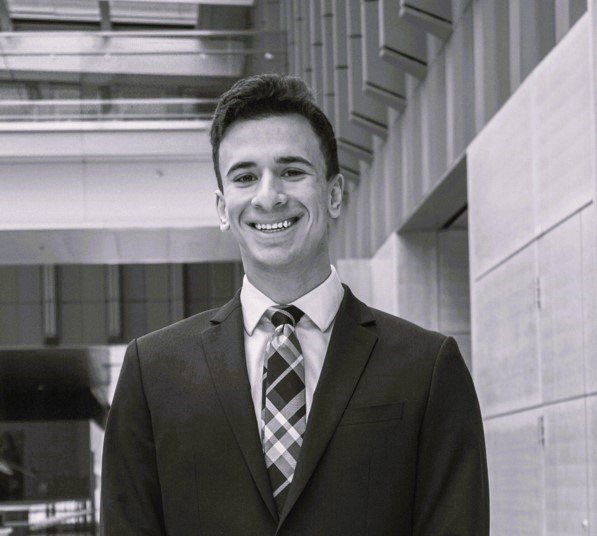
\includegraphics[width=0.4\linewidth]{rtberger}

\hypertarget{adam-zhang}{%
\section{Adam Zhang}\label{adam-zhang}}

Hi! I'm Adam Zhang. I am a Master of Business Analytics student at the Ross School of Business at University of Michigan. I attended University of Illinois Urbana-Champaign where I majored economics for undergrad. I enjoy cooking, watching movies, listening to musics (mainly 70s and 80s), and going to art museums.


\includegraphics[width=0.4\linewidth]{AZ}

\hypertarget{michelle-xu}{%
\section{Michelle Xu}\label{michelle-xu}}

Hello, I'm Michelle Xu, originally from China. I spent six years living in the beautiful city of San Diego, California. After high school, I moved to Ann Arbor, Michigan, to pursue a major in Bioinformatics at LS\&A. Currently, I'm a Master of Business Analytics student at the University of Michigan, Ross School of Business.

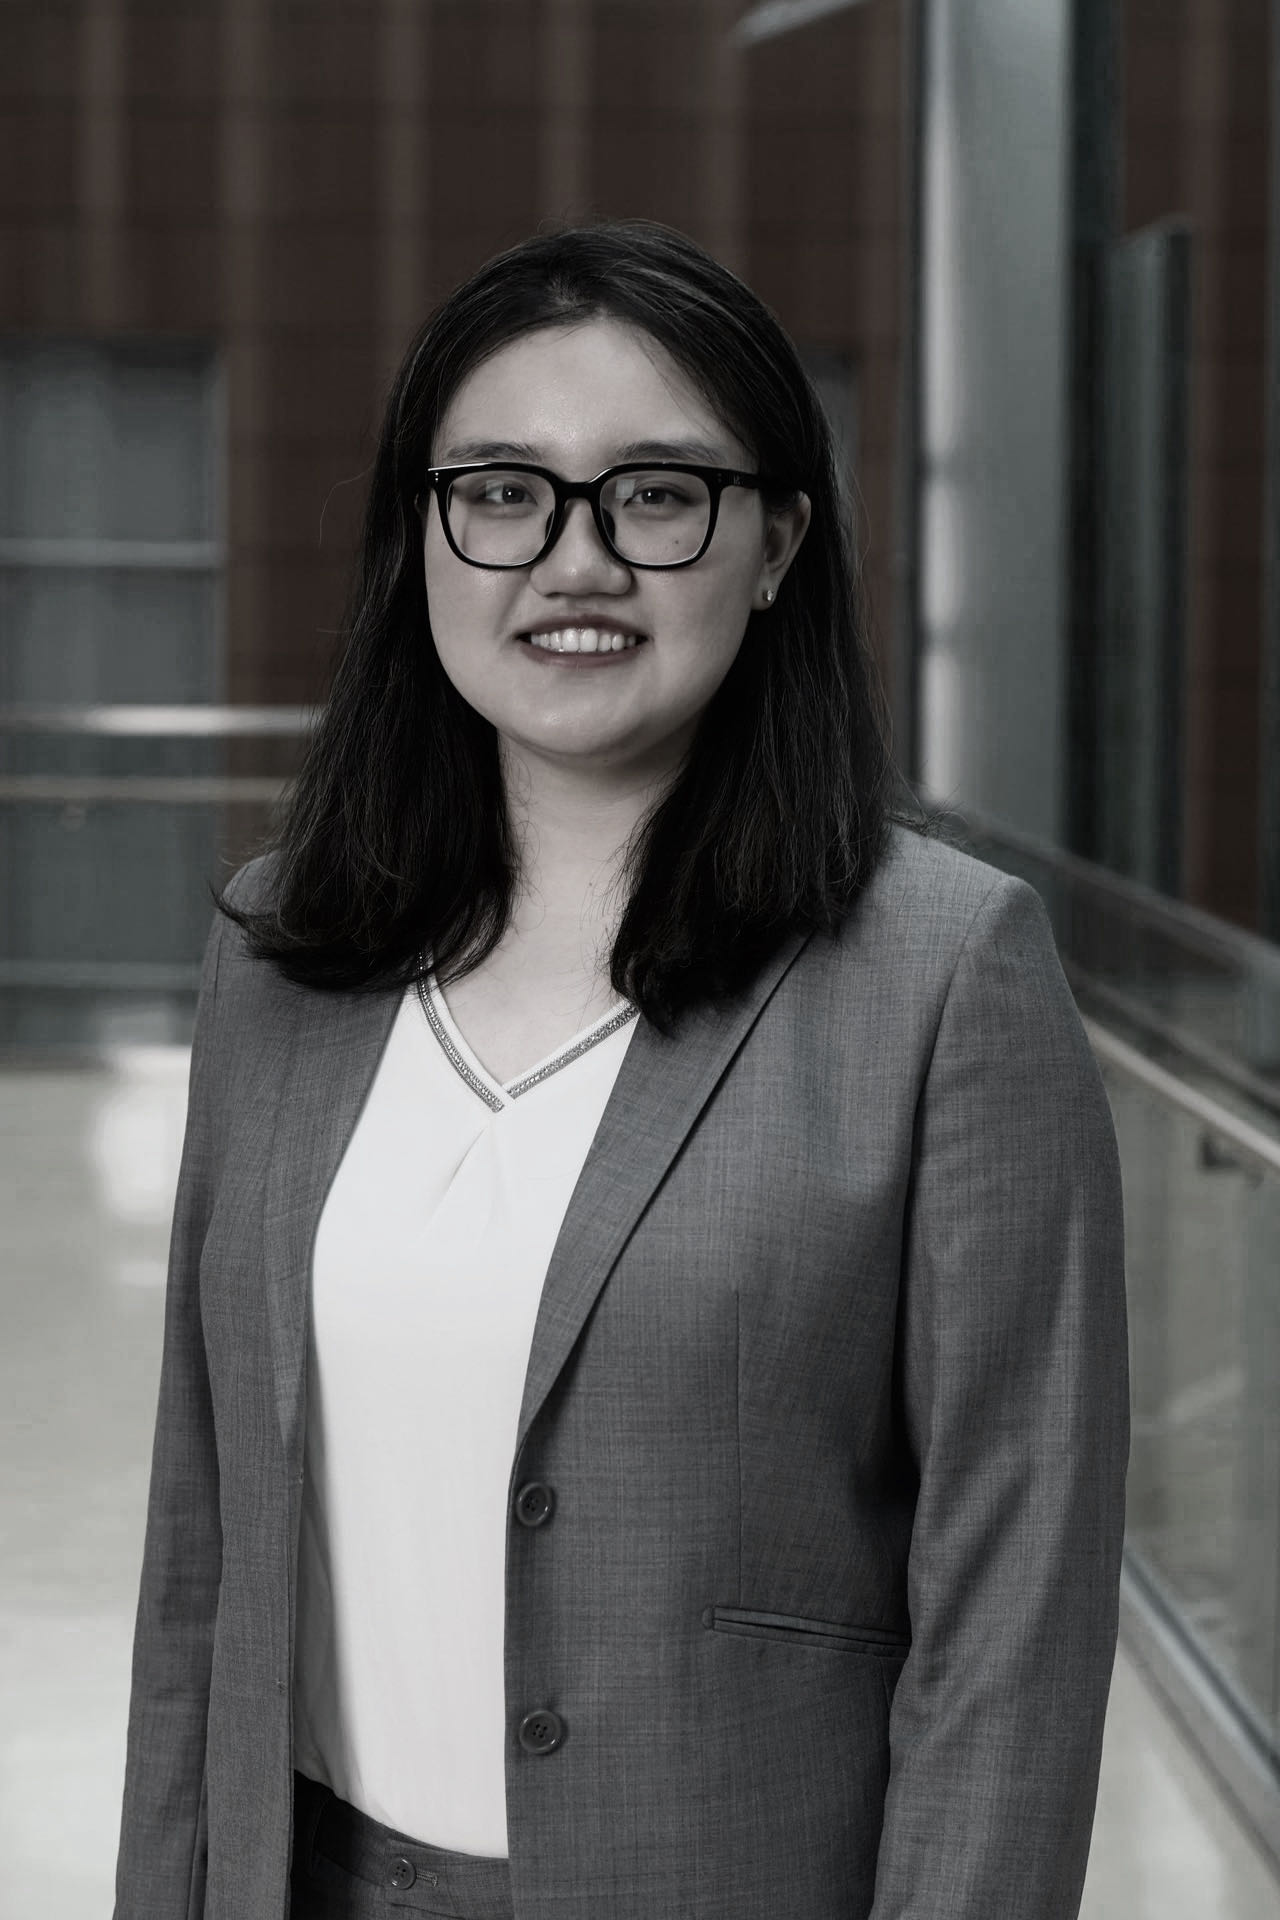
\includegraphics[width=0.4\linewidth]{WechatIMG10}

\hypertarget{sona-coshal}{%
\section{Sona Coshal}\label{sona-coshal}}

Hi, my name is Sona! I'm born and raised in Columbia, South Carolina and a proud USC Gamecock! I have a BSBA in Finance and Supply Chain from the Darla Moore School Business.


\includegraphics[width=0.4\linewidth]{Sona's_Photo}

\hypertarget{fuad-chedid}{%
\section{Fuad Chedid}\label{fuad-chedid}}

Hi! I'm Fuad, a native Michigander! Before joining the Master of Business Analytics program at Michigan Ross, I was based in Dubai, UAE, and worked in the energy sector. I consider myself a ``tech head'' and my main area of interest is the intersection of business and technology. I enjoy travelling and so far have visited 27 countries and five continents.

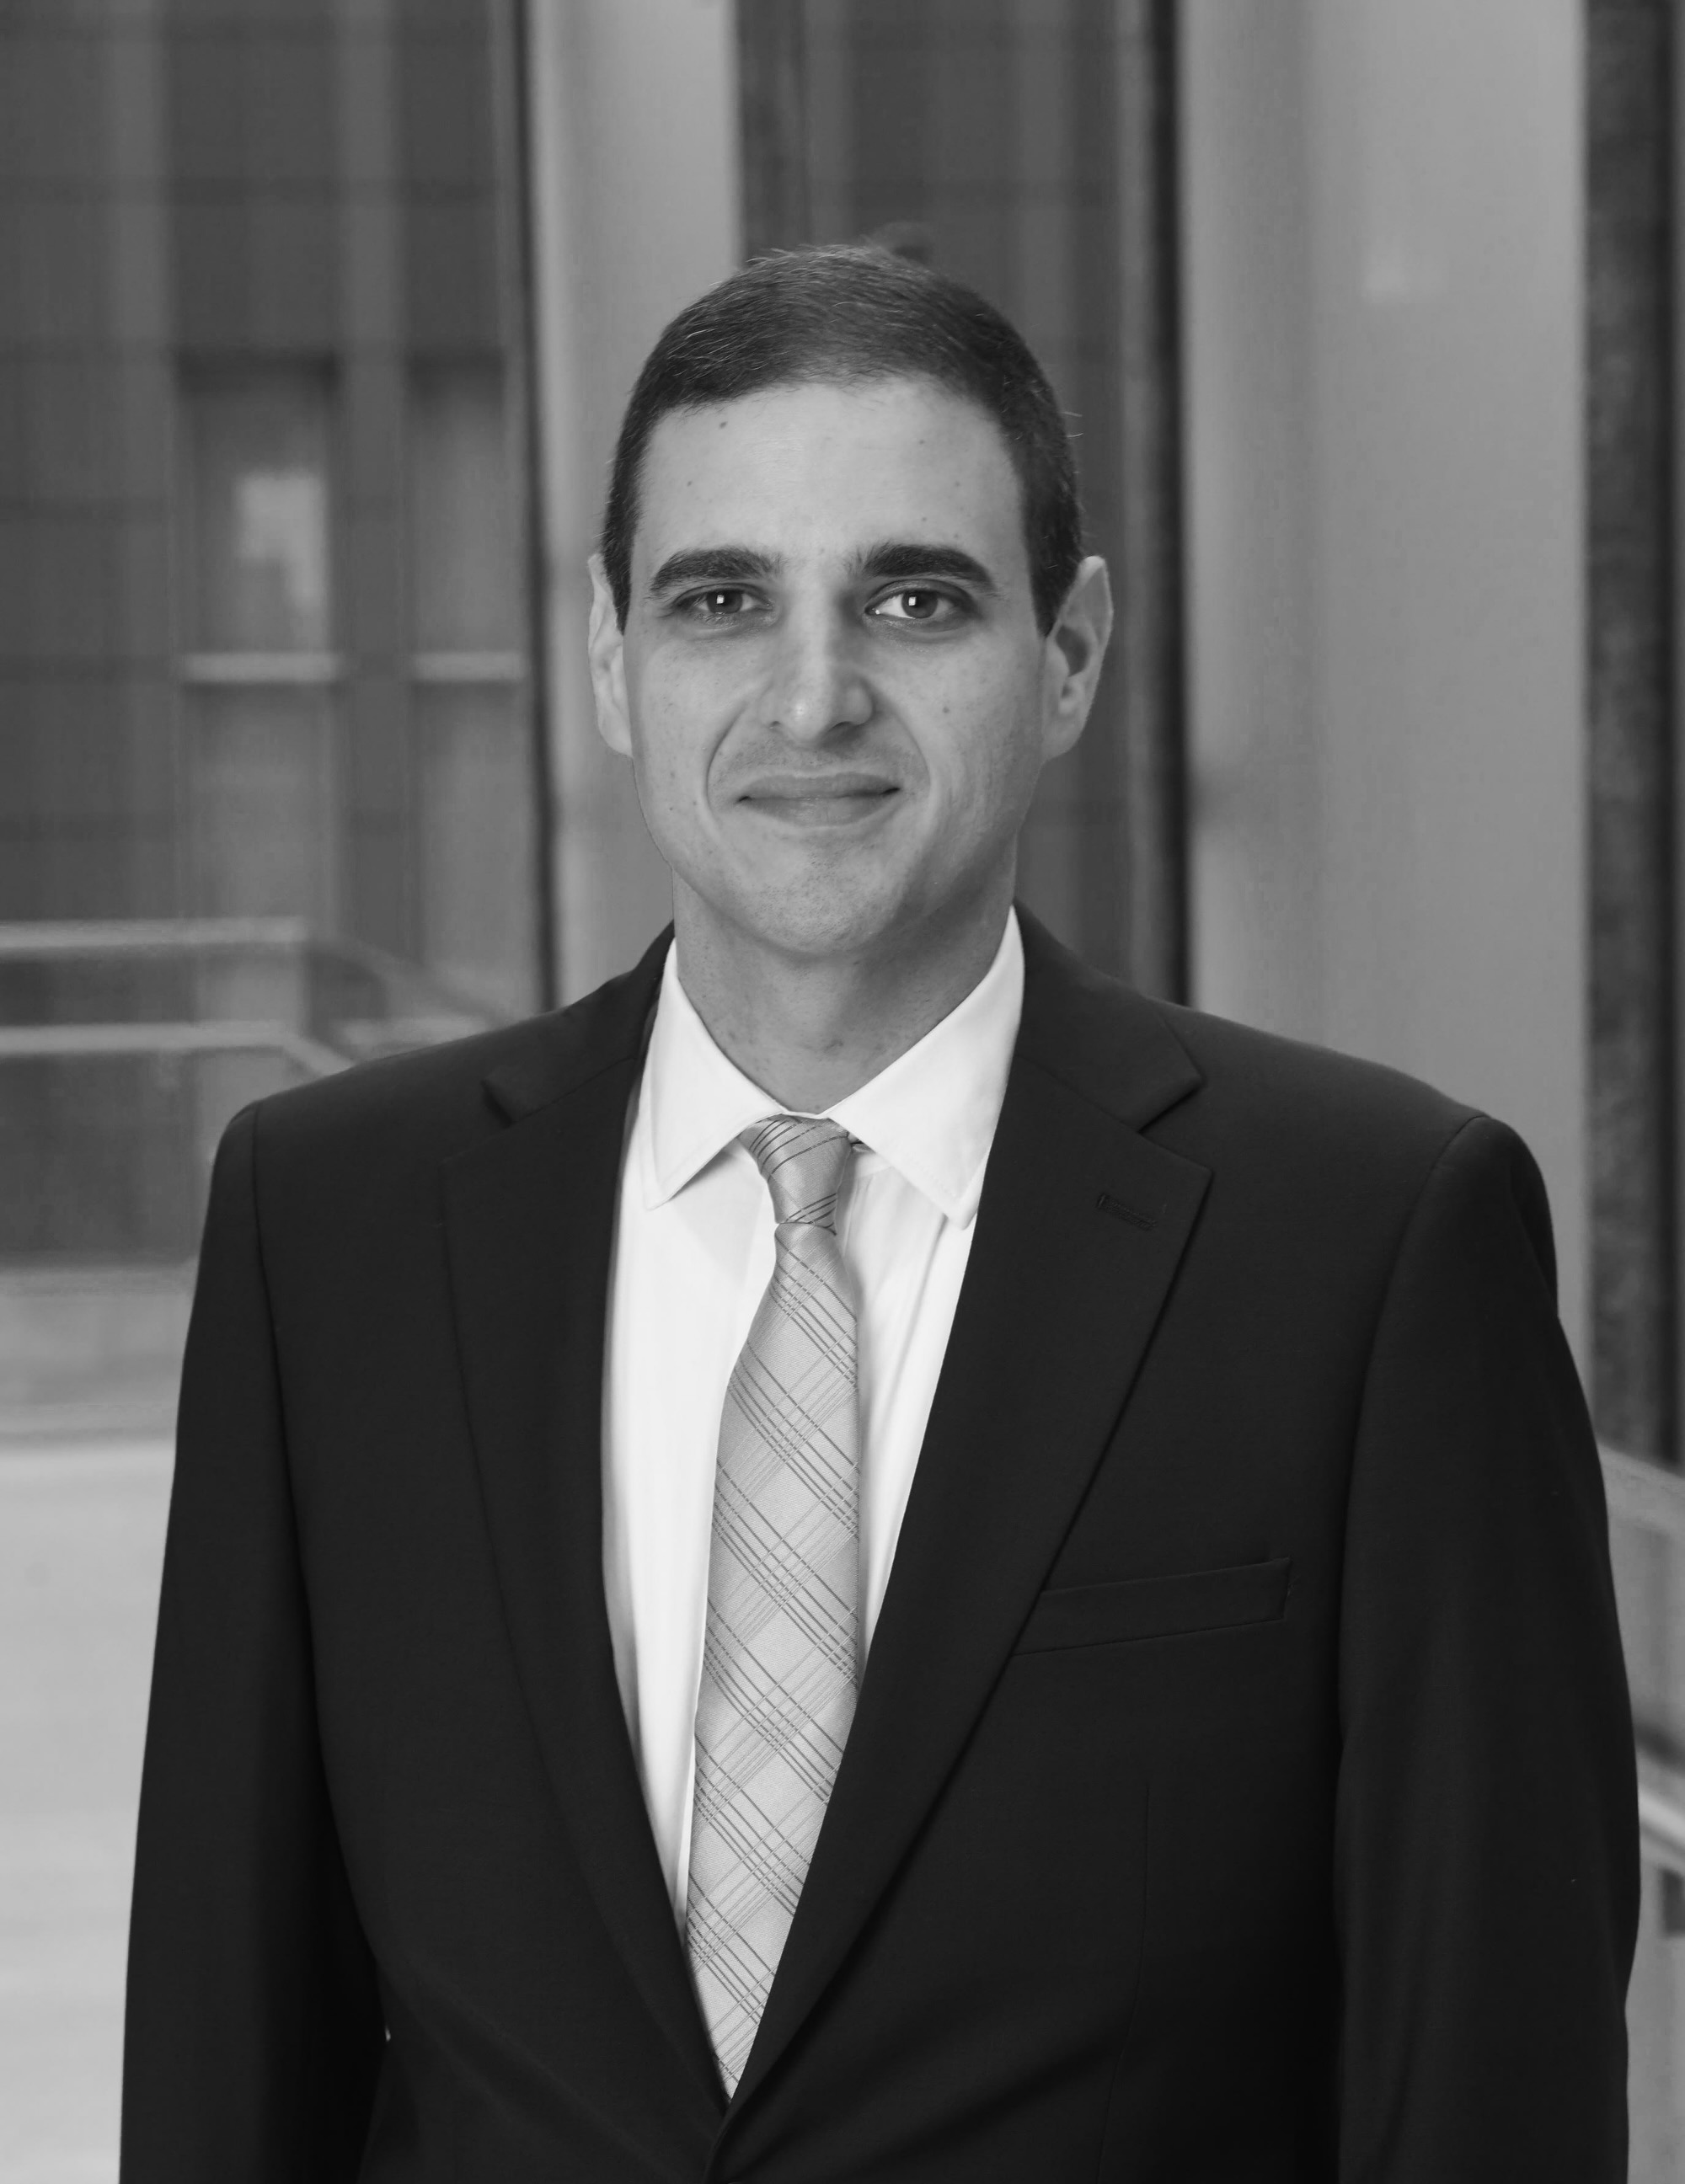
\includegraphics[width=0.4\linewidth]{fpic}

\hypertarget{ross-faculty-perspective}{%
\chapter{Ross Faculty Perspective}\label{ross-faculty-perspective}}

Faculty and Staff are uniquely positioned to provided perspective on the opportunities and challenges faced in higher education in the age of GenAI. Several questions come to mind, and to gain insight, we conducted five interviews with the aim of drawing insight from the responses.

\hypertarget{participants}{%
\section{Participants}\label{participants}}

\begin{longtable}[]{@{}
  >{\centering\arraybackslash}p{(\columnwidth - 8\tabcolsep) * \real{0.1340}}
  >{\centering\arraybackslash}p{(\columnwidth - 8\tabcolsep) * \real{0.2775}}
  >{\centering\arraybackslash}p{(\columnwidth - 8\tabcolsep) * \real{0.1914}}
  >{\centering\arraybackslash}p{(\columnwidth - 8\tabcolsep) * \real{0.2488}}
  >{\centering\arraybackslash}p{(\columnwidth - 8\tabcolsep) * \real{0.1340}}@{}}
\toprule\noalign{}
\endhead
\bottomrule\noalign{}
\endlastfoot
\textbf{Ross Staff} & \textbf{Dr.~John Branch} & \textbf{Dr.~Ali Hojjat} & \textbf{Dr.~John Silberholz} & \textbf{U-M Professor} \\

\includegraphics[width=1.04167in,height=\textheight]{plc.png} & 
\includegraphics[width=1.04167in,height=\textheight]{branch.jpeg}

Clinical Associate Professor of Business Administration

Michigan Ross & 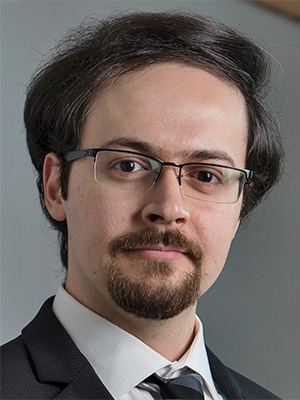
\includegraphics[width=1.04167in,height=\textheight]{hojjat.jpeg}

Lecturer of Technology and Operations

Michigan Ross & 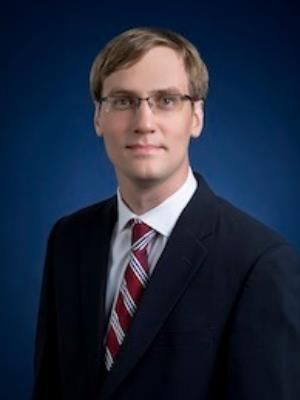
\includegraphics[width=1.04167in,height=\textheight]{silverholtz.jpeg}

Assistant Professor for Technology and Operations

Michigan Ross & 
\includegraphics[width=1.04167in,height=\textheight]{plc.png} \\
\end{longtable}

\hypertarget{qa}{%
\section{Q\&A}\label{qa}}

Interviews were conducted individually, and the below responses to each question are \textbf{paraphrased}.

\textbf{Question:} \emph{Do you foresee any challenges or opportunities that AI advancements could bring to the business school environment? Are there any potential risks or rewards associated with increasing the integration of AI in student learning? Have you observed any specific improvements in student learning outcomes or performance when using AI tools in the classroom?}

\begin{longtable}[]{@{}
  >{\raggedright\arraybackslash}p{(\columnwidth - 2\tabcolsep) * \real{0.0270}}
  >{\raggedright\arraybackslash}p{(\columnwidth - 2\tabcolsep) * \real{0.9730}}@{}}
\toprule\noalign{}
\endhead
\bottomrule\noalign{}
\endlastfoot
\textbf{Ross Staff} & Beyond academic integrity, AI has disrupted other aspects of higher education. For example, fraudulent applications are a main concern. Admission essays could be written using AI tools, or applicants may hire consultants. This raises questions on the effectiveness of requiring admission essays and places more weight on direct interviews. During an interview, the applicant could be asked to define a made-up word, and the goal isn't to make up a definition but to admit that you do not know what it means. Increasingly, applications are becoming more about determining who's authentic. Historically, essay evaluation has been a long-standing issue, but the advent of GenAI compounds the problem. Everyone can look good on paper, but the intention behind essays is to understand an applicant's traits and personality. As a response, interviews can carry more weight during our application evaluation. \\
\textbf{Dr.~Ali Hojjat} & ChatGPT is a great supplemental tool for teaching business analytics. This work in general requires a great deal of high-level synthesis and critical thinking skills. These are areas that ChatGPT does not provide much assistance. On the other hand, GenAI tools like ChatGPT can help students with the rote learning associated with advanced analytics, such as memorizing syntax and generating starter codes from which to work. All in all, these tools allow students to be more efficient in their learning, without compromising the ability to understand and solve problems in a practical sense. There are some concerns with low-level analytical courses such as undergraduate Excel classes where students can copy and paste directly from ChatGPT and generally score well. But intermediate and advanced analytical work within Excel or other tools requires a great deal of synthesis and abstraction, which are not strengths of GenAI tools. \\
\textbf{Dr.~John Branch} & GenAI is just another tool, and it is here to stay. We ought to get out in front of it and integrate it into our teaching. During a recent emergency faculty meeting, we discussed our response strategy to the proliferation of GenAI in higher education. A major concern was academic integrity. Specifically, for writing-intensive courses like those which I teach, a large concern is that students would submit their work through the dependent use of GenAI tools. \\
\textbf{Dr.~John Silberholz} & GenAI is a positive development in academia. I don't see any concerns with the development of our students and the skills that they need to be successful in the workplace. The recent GenAI developments are akin to the rise of search engine prominence. Those who knew of the technology and understood how to use it benefited in the short term. But eventually, that advantage dissipates as the tool becomes more widespread in its use. The biggest challenge from an academic perspective is the ability to ensure equity of access to all students. This will be particularly challenging as these tools advance and become more specialized. In today's classroom, GenAI tools allow students to focus on higher learning principles that require critical thinking skills by offloading the mental capacity needed to process lower-level memorization work. \\
\textbf{U-M Professor} & GenAI has brought more opportunities than challenges to higher education. Inevitably, it is a tool that will be with all of us for the rest of our lives. We must learn to live in the AI world, and anticipate future developments. One significant challenge is that certain skills will no longer be marketable to employers, and we have to adjust how we prepare students to enter the workforce. Although it can be difficult to let go of past learning objectives, if ChatGPT can do it, why teach it? However, when it comes to coursework that involves critical thinking and problem-solving, GenAI poses no significant threat to learning objectives. Instructors need to be explicit at the start of the course and lay out the ground rules for GenAI tool use. \\
\end{longtable}

\textbf{Question:} \emph{How can educators maintain academic integrity when students have access to AI language models that can generate text and answers?}

\begin{longtable}[]{@{}
  >{\raggedright\arraybackslash}p{(\columnwidth - 2\tabcolsep) * \real{0.0267}}
  >{\raggedright\arraybackslash}p{(\columnwidth - 2\tabcolsep) * \real{0.9733}}@{}}
\toprule\noalign{}
\endhead
\bottomrule\noalign{}
\endlastfoot
\textbf{Ross Staff} & Instructors have to fundamentally change the way that they teach. GenAI tools are incredibly useful for developing solutions and will continue to be leveraged throughout society. Professors need to evaluate a student's comprehension and ability to understand concepts through a dynamic and critical lens. Static representations of a student's understanding are no longer acceptable means of demonstrating comprehension. There is an apparent rift between faculty that believe in changing the way they teach with new technology and those that do not. \\
\textbf{Dr.~Ali Hojjat} & Academic integrity should be defined as incidents where individuals have access to resources that others didn't. As long thet access to GenAI tools remains consistent across the academic setting, it shouldn't be seen as a complicating factor contributing to an unfair disadvantage for one group against another. The greater risk to academic development lies within specific fields such as humanities and English, where a large portion of the curriculum overlaps with the core competencies associated with GenAI tools. To combat this, professors need to ensure that their coursework is delivered in a format that doesn't permit excessive use of online resources. It is important to make sure that the questions on exams and homework require critical thinking. In fact, in certain courses, GenAI is encouraged! I'd rather students spend less time memorizing coding syntax and more time developing critical business insight skills. \\
\textbf{Dr.~John Branch} & Examples of academic integrity issues are common: the Community Values Committee manages new infractions every week. Even within BA500, we have seen cases of subpar performance due to GenAI dependence.~ We are developing our policies to address these issues and, and are heading towards a future with fewer and fewer infractions. \\
\textbf{Dr.~John Silberholz} & The onus of academic integrity lies on the professors and revolves around their ability to create and structure a class that allows students to explore tools such as GenAIs, without compromising their conceptual understanding of the subject matter. In-person assessments that focus on critical thinking skills need to comprise the bulk of the graded work to ensure that students understand and can apply the learnings. Instructors should test their assignments using GenAI tools to evaluate if any learning objectives are compromised and place more emphasis on critiquing student outputs. Professors that don't revise their curriculum for the GenAI era will witness diminishing returns on their educational value. GenAI is not going away. Academia needs to take advantage of the new resources made possible by advancements in technology and adjust their content and teaching methods to account for the changing environment. \\
\textbf{U-M Professor} & Academic integrity issues are not new, and GenAI tools are not going to have a major effect on this topic. Even though there is no accurate way to detect usage, ChatGPT and other similar tools are not guaranteed to deliver coherent and correct answers. Anyone who uses these tools has to evaluate and improve the output before submitting a final answer. Professors evaluate students holistically, their writing voice from previous work, how they speak and interact in class, etc. As long as the student understands the information provided by the GenAI tool, he or she should be free to copy and paste directly from the source and use it without modification. It's up to the professor to construct an evaluation process that doesn't slow down the learning process. If a student can speak intelligently about a topic and can participate in a socratic discussion, is a written essay really necessary to demonstrate understanding and application? \\
\end{longtable}

\textbf{Question:} \emph{What are some effective ways to integrate AI tools into the business school curriculum to enhance the learning experience? Are there any specific subjects or topics where AI can be particularly valuable for students?}

\begin{longtable}[]{@{}
  >{\raggedright\arraybackslash}p{(\columnwidth - 2\tabcolsep) * \real{0.0254}}
  >{\raggedright\arraybackslash}p{(\columnwidth - 2\tabcolsep) * \real{0.9746}}@{}}
\toprule\noalign{}
\endhead
\bottomrule\noalign{}
\endlastfoot
\textbf{Ross Staff} & Higher education is an interesting beast. Professors have unique jurisdiction over their classes, specifically on whether using AI is allowed in their classes. There are lots of school policies in place, but in the end, it is the professors who are in charge. However, because of varied faculty opinions on how these tools should be used for coursework, it can lead to a frustrating student experience due to inconsistent guidelines. \\
\textbf{Dr.~Ali Hojjat} & The value of tools like ChatGPT resides in the ability to focus on the ``why'' and less on the ``dry'' component of learning, such as syntax and manual calculation. Classes such as Python 101 should be taught in conjunction with ChatGPT, as GenAI tools such as programming co-pilots will be widely used within the workforce. In addition to the practical considerations of professional life, students can learn more, faster, and generate a greater level of understanding in a shorter amount of time when leveraging modern productivity-enhancing tools. Assignments should not be simply to summarize content, but they should require students to understand, review, edit, and clean up any GenAI output. Einstein once posited that the education system is set up to memorize facts, but the goal is to teach students how to think and analyze. If someone were to ask him ``What's the speed of sound?'' Einstein would respond that ``I don't keep such information in my brain that is readily available in books.'' \\
\textbf{Dr.~John Branch} & For many years, education (business schools) have been struggling with isolation vs.~integration. Isolation is defined as a topic so critical that it needs its own course - and an expert in the field should teach it. Integration is for learning objectives that should be in all courses due to universality - and assumes a degree of expertise in the professor. Some examples of previous hot topics that have this inflection point about integration or isolation have been globalization, corporate social responsibility, e-commerce, and more. So, it needs to be determined whether we create a new class or integrate it into all classes. \\
\textbf{Dr.~John Silberholz} & GenAI tools solve the ``blank page'' problem, but they do not bring students to the highest level of understanding without critical thinking work that is currently beyond the limits of GenAI. These tools are best used to generate material as a starting point for an activity or assignment as they can handle prompts across an unlimited number of academic and professional disciplines. Despite their great efficacy and flexibility, these tools do not generate a final finished product worthy of scrutiny without additional and thoughtful work performed by its users. Instructors need to integrate GenAI into the coursework where it can add value. By experimenting with these tools while designing the curriculum, we can enhance and improve learning outcomes for students. \\
\textbf{U-M Professor} & GenAI tools can enhance the learning experience by allowing students to focus on critical thinking frameworks and problem-solving methodology. We also need to be cognizant of equitable access to avoid disparity. As the workplace continues to outsource repetitive tasks to AI, the requirement that students memorize or understand the minutiae of every task diminishes. If a GenAI tool can complete an assignment or perform a task at a passable level within a matter of seconds, then why ask our students to learn and develop those skills? In reality, most industries and professional settings dictate the use of time-saving and productivity-enhancing tools and constructs. Those who continue to perform non-value add tasks manually will eventually fall behind. Professors need to ask themselves whether they are asking students to acquire information for the sake of learning, or whether they are teaching students the skills and conceptual understandings needed to succeed in their futures. \\
\end{longtable}

\textbf{Question:} \emph{What do you envision as the future role of AI in business education, and how might it evolve in the coming years?}

\begin{longtable}[]{@{}
  >{\raggedright\arraybackslash}p{(\columnwidth - 2\tabcolsep) * \real{0.0333}}
  >{\raggedright\arraybackslash}p{(\columnwidth - 2\tabcolsep) * \real{0.9667}}@{}}
\toprule\noalign{}
\endhead
\bottomrule\noalign{}
\endlastfoot
\textbf{Ross Staff} & The application expands thinking, but it's terrifying. It's similar to social media in stunting communication and thinking ability; it is that piece of humanity that might be concerning or missing from future generations where AI is ubiquitous. AI will be applicable in nearly all classes. Kids can utilize AI tools as a tutor, and it will only get better and better. \\
\textbf{Dr.~Ali Hojjat} & It holds a transformative potential, evolving to enhance students' learning experiences and skill development. GenAI tools like ChatGPT can serve as invaluable supplements for teaching business analytics, addressing specific learning needs. While ChatGPT may not directly support high-level synthesis and critical thinking, it excels at aiding students in rote learning aspects of advanced analytics. By assisting with tasks such as memorizing syntax and generating starter codes, GenAI tools enable students to become more efficient learners without compromising their problem-solving abilities. However, it's essential to be mindful of the potential pitfalls in certain contexts, such as allowing excessive reliance in lower-level analytical courses. \\
\textbf{Dr.~John Branch} & Regardless of how good AI gets, it's not the tool that makes the learning, like with Khan Academy and other similar tools. Will AI get better and better? Sure. But will it get to a point where it can teach like me? Maybe not. \\
\textbf{Dr.~John Silberholz} & Despite the rapid advancements in AI in the past few years, I don't expect GenAI tools to advance so quickly that within the next 5 years, we would witness a significant degradation in real-world skills caused by the proliferation of GenAI tools and capabilities. Entry-level job duties will most likely shift during this time, and academia will have to adjust accordingly. As teaching and learning models adapt to the changes in technology, certain skills become less and more useful. As long as teachers and students adapt and focus on the learning outcomes needed to perform effectively in the workforce, we shouldn't be concerned about the negative effects of GenAI tools. \\
\textbf{U-M Professor} & Currently, I don't envision Generative AI as a major threat to the way people learn and process information. GenAI is essentially a pattern-matching tool that predicts the next best possible word based on some input text. It only has the ability to re-combine old information in a manner that it perceives to be beneficial. This is different from General AI which possesses the ability to mimic human thinking. The watershed moment in academic and human history will occur when advancements in General AI allow these programs to replace the basic cognitive reasoning skills which currently differentiate man from machine. \\
\end{longtable}

\hypertarget{insights}{%
\section{Insights}\label{insights}}

Based on our interviews with faculty and staff at the Ross School of Business, while there is a need for change in the way that educators need to teach with the use of AI by the student population, we must also acknowledge that instructors are autonomous in how they decide to shape their courses and policies. There needs to be a greater consensus by the school as a whole to avoid complications between classes as students utilize this tool because of its efficiency, competency, and overall value that it adds to the day-to-day learning process.

Among the recurring themes, it has been emphasized that detecting AI-generated content, particularly in generative AI, poses a challenge for educators that believe it violates academic integrity in their classes. Specifically, there are heightened risks for writing-intensive, humanities courses, but more opportunities and possibilities for more technical disciplines, illustrating how divisive this powerful tool can be.

A noticeable divide has become evident between faculty members who enthusiastically embrace AI's potential and those who have reservations about its use, highlighting the need for constructive dialogue across the school to bridge this gap. As we progress, it is evident that education must adapt to the evolving technological landscape. The use of AI as a tool for students and educators alike will only increase, and so there is a dire need for steps toward this evolution in teaching methodologies to prioritize conceptual comprehension over rote memorization. Students need to cultivate critical thinking and problem-solving skills as future business leaders in a digitized era, rather than regurgitation of information that will become generally useless after the class has ended.

Lastly, there is a consensus that AI will only improve as investment skyrockets into the new technology. As we navigate the ever-evolving landscape of AI, the Ross School of Business is poised to harness its benefits while navigating the nuances and challenges that come with this transformative tool in business education and at the University of Michigan as a whole.

\hypertarget{current-state-of-affairs}{%
\chapter{Current State of Affairs}\label{current-state-of-affairs}}

Since the proliferation of publicly available generative AI in November 2022, U-M has been positioning itself to respond and adapt. Undoubtedly, there is a need for institutional understanding and action to ensure that generative AI is leveraged in support of the University's mission. This section provides information on the currently published university-wide guidance.

\hypertarget{u-m-genai-website}{%
\section{U-M GenAI Website}\label{u-m-genai-website}}

Recently established by the GAIA Committee (see \ref{gaia-committee}), \url{https://genAI.umich.edu} is a comprehensive resource containing the latest guidance and information for all members of the U-M community.

\hypertarget{gaia-committee}{%
\section{GAIA Committee}\label{gaia-committee}}

The Generative AI Advisory (\href{https://it.umich.edu/strategy-planning/gaia}{GAIA}) Committee was established in the first half of 2023, with the overall aim being:

\begin{quote}
``to provide guidance to the university community for the use of generative AI and provide strategic advice to the~VPIT-CIO~and Provost.''
\end{quote}

An overview of the committee's \href{https://genai.umich.edu/committee-report}{official report}, published on June 30th 2023, is provided in section \ref{initial-report-june-30-2023}.

The committee currently includes members from the following schools, colleges, and departments:

\begin{longtable}[]{@{}ll@{}}
\toprule\noalign{}
School / College / Department & \# of Member(s) \\
\midrule\noalign{}
\endhead
\bottomrule\noalign{}
\endlastfoot
\textbf{Executive Sponsor} & 1 \\
\textbf{College of Engineering} & 4 \\
\textbf{Medical School} & 2 \\
\textbf{School of Public Health} & 1 \\
\textbf{College of Literature, Science, and the Arts} & 3 \\
\textbf{School of Education} & 2 \\
\textbf{School of Information} & 2 \\
\textbf{Ross School of Business} & 2 \\
\textbf{Information and Technology Services} & 1 \\
\textbf{Center for Research on Learning and Teaching} & 1 \\
\textbf{Center for Academic Innovation} & 1 \\
\textbf{Office of the Provost for DE\&I} & 1 \\
\textbf{U-M Flint} & 1 \\
\textbf{U-M Dearborn} & 1 \\
\end{longtable}

\emph{As of Aug 2023. Note: Some members represent more than one affiliation.}

\hypertarget{initial-report-june-30-2023}{%
\subsection{Initial Report (June 30 2023)}\label{initial-report-june-30-2023}}

The below extracts from the \href{https://genai.umich.edu/committee-report}{report} have been selectively chosen based on their immediate relevancy to instructors.

\hypertarget{overall-recommendations}{%
\subsubsection*{Overall Recommendations}\label{overall-recommendations}}
\addcontentsline{toc}{subsubsection}{Overall Recommendations}

A brief highlight of the overarching recommendations:


\includegraphics[width=0.3125in,height=0.20833in]{open.png}

\begin{quote}
\begin{itemize}
\item
  Dissemination of guidance and launch of campus discussion (Timeline: immediate).
\item
  Teaching, Learning, and Academic Innovation (Timeline: Fall 2023). U-M can approach GenAI as an opportunity to rethink how we teach and define meaningful learning objectives, promote inclusion and equity, and assess learning. \textbf{Instructors should be given complete flexibility to allow or disallow the use of GenAI tools.}
\item
  Assess the use of GenAI in research and set best practice standards for privacy protections; data use controls; and updating research integrity reated SPGs, PEERS modules, and RCR training.
\item
  Provost, VPR and VPIT should establish a U-M wide research initiative in the area of Generative AI (Timeline: Fall 2023/Winter 2024).

  \begin{itemize}
  \tightlist
  \item
    U-M should consider developing its own version of foundation GenAI models to enable research and innovation (Timeline: Begin activities in Fall 2023).
  \end{itemize}
\item
  Expansion of IT infrastructure to accommodate secure and equitable access to GenAI plat- forms and tools (Timeline: Immediate and Variable).

  \begin{itemize}
  \tightlist
  \item
    Create and deliver new GenAI services. These services will be offered across three tiers, each catering to different needs and technical proficiencies and made available to Ann Arbor, Flint, and Dearborn.
  \end{itemize}
\item
  VPIT to work with the GAIA committee to coordinate and establish an AI digital commons where our community can share best practices and emerging ideas in GenAI (Timeline: Immediate).
\item
  Launch a U-M GenAI website providing strategy, policies, resources, and links. Coordinate this with a well-defined communication plan (Timeline: Immediate).
\end{itemize}
\end{quote}


\includegraphics[width=0.3125in,height=0.20833in]{close.png}

\hypertarget{key-benefits-and-opportunities}{%
\subsubsection*{Key Benefits and Opportunities}\label{key-benefits-and-opportunities}}
\addcontentsline{toc}{subsubsection}{Key Benefits and Opportunities}

Highlights of key benefits and opportunities:


\includegraphics[width=0.3125in,height=0.20833in]{open.png}

\begin{quote}
\begin{itemize}
\item
  GenAI will enable U-M to advance its mission and accelerate and support Vision 2034.
\item
  GenAI has the potential to transform teaching outcomes by creating customizable learning pathways
\item
  GenAI will accelerate knowledge development,including rethinking of disciplinary boundaries and domains, and possibly, defining new ones.
\item
  From an efficiency perspective, GenAI has the potential to support enhanced administrative productivity and service quality throughout the University.
\item
  \textbf{U-M has the intellectual depth, resources, and international and national connections and networks to be the leader in the development and appropriate use of GenAI.}
\end{itemize}
\end{quote}


\includegraphics[width=0.3125in,height=0.20833in]{close.png}

\hypertarget{key-threats-and-weaknesses}{%
\subsubsection*{Key Threats and Weaknesses}\label{key-threats-and-weaknesses}}
\addcontentsline{toc}{subsubsection}{Key Threats and Weaknesses}

Highlights of key threats and weaknesses:


\includegraphics[width=0.3125in,height=0.20833in]{open.png}

\begin{quote}
\begin{itemize}
\item
  Several technical weaknesses currently exist, including temporal ignorance, hallucination and fabrication, misattribution, overriding safety protocols, inadvertent inclusion breaches or ethical problems, and bias in training data.
\item
  Social weaknesses refer to those that arise from the interaction between the system and user, which may yield unanticipated actions and outcomes. While myriad and evolving, a few examples of social weaknesses include

  \begin{itemize}
  \item
    rapid escalation of deep fakes in video and audio,
  \item
    user attribution of output generated by GenAI to themselves or others,
  \item
    GenAI companion giving dangerous advice to children,
  \item
    use of GenAI to perform research without appropriate disclosure,
  \item
    inappropriate use of prompt data by AI provider,
  \item
    reduced demand for human labor in many professions,
  \item
    inequitable access to state-of-the-art GenAI systems,
  \item
    and unauthorized generation or replication of copyrighted or otherwise protected material.
  \end{itemize}
\end{itemize}
\end{quote}


\includegraphics[width=0.3125in,height=0.20833in]{close.png}

\hypertarget{instructor-recommendations}{%
\subsubsection*{Instructor Recommendations}\label{instructor-recommendations}}
\addcontentsline{toc}{subsubsection}{Instructor Recommendations}

The committee's initial report identifies teaching and learning as the most \emph{``immediate and significant GenAI application domain''} and provides guidance to instructors to help prepare for the Fall 2023 semester. The below sections include highlights of the guidance.

Generally, the committee finds that it is presently ``nearly impossible to enforce'' banning GenAI use in coursework. And therefore, strongly recommends that instructors consider the following questions when adapting course work:


\includegraphics[width=0.3125in,height=0.20833in]{open.png}

\begin{quote}
\begin{itemize}
\item
  Should GenAI be used in the course or not---and why or why not?
\item
  If GenAI is to be used, how is the use to be documented?
\item
  Should course learning objectives be revised?
\item
  Should GenAI competencies be taught in the specific disciplinary context?
\item
  Should assessments be revised?
\end{itemize}
\end{quote}


\includegraphics[width=0.3125in,height=0.20833in]{close.png}

\hypertarget{genai-permit-or-ban}{%
\paragraph*{GenAI: permit or ban?}\label{genai-permit-or-ban}}
\addcontentsline{toc}{paragraph}{GenAI: permit or ban?}

The report also addresses the fact that current academic misconduct definitions, Honor Codes, and academic integrity policies do not account for GenAI explicitly, and should be updated. The committee also acknowledges that students who use GenAI in an unauthorized manor may be committing cheating or plagiarism.

In determining GenAI permissability within academic misconduct policies, the report provides the following view:


\includegraphics[width=0.3125in,height=0.20833in]{open.png}

\begin{quote}
Common approaches to updating academic misconduct policies are:

\begin{itemize}
\item
  Determining that ChatGPT (or GenAI) is prohibited help from another ``person'' (e.g., UCLA),
\item
  Defining GenAI as a ``source'' that should be acknowledged (e.g., UW Madison).
\end{itemize}

The GAIA committee believes that the ``person'' approach misleadingly attributes sentience and a reasoning capacity to GenAI, and proposes that the ``source'' approach is more workable, and aligned with our mission of teaching students to engage effectively and ethically with the world around them.
\end{quote}


\includegraphics[width=0.3125in,height=0.20833in]{close.png}

With regard to course policy, the report provides the following guidance to instructors:


\includegraphics[width=0.3125in,height=0.20833in]{open.png}

\begin{quote}
\begin{itemize}
\item
  it is critical that expectations are clearly articulated in the syllabus and continually reinforced when assignments are given.
\item
  \textbf{instructors should be given flexibility to allow or disallow the use of GenAI tools. If the latter approach is adopted, the committee discourages the use of surveillance and plagiarism detection tools as they cannot be reliably counted upon at the present moment.}
\item
  GenAI is changing rapidly, and new tools will become available. Course policies therefore need to be provisional and subject to change.
\end{itemize}

Course policies might fall into one of three categories:

\begin{itemize}
\item
  Specific uses of GenAI are encouraged (generating ideas, editing, translating, outlining).
\item
  Specific uses of GenAI are allowed if students clearly distinguish between their original work and GenAI output (highlighting output, tracking changes in GenAI output).
\item
  Any use of GenAI constitutes academic misconduct.
\end{itemize}

If GenAI tools are allowed, the instructor should be clear which tools are allowed and in what capacity. On the other hand, if GenAI tools are disallowed, the committee suggests that the instructor give reasons why the use of GenAI tools would hinder learning.
\end{quote}


\includegraphics[width=0.3125in,height=0.20833in]{close.png}

The report also suggests instructors review recommendations from \url{http://sentientsyllabus.org} for items to consider including in the syllabus.

\hypertarget{redesigning-coursework}{%
\paragraph*{Redesigning Coursework}\label{redesigning-coursework}}
\addcontentsline{toc}{paragraph}{Redesigning Coursework}

The committee recommends that, out the outset, instructors become familiar with and practice using GenAI tools. For information regarding currently available tools, see section \ref{publicly-available-generative-ai}.

Once familiarized, the committee recommends that instructors consider the following with respect to their current course design:


\includegraphics[width=0.3125in,height=0.20833in]{open.png}

\begin{quote}
\begin{enumerate}
\def\labelenumi{\arabic{enumi}.}
\item
  What are the course objectives and rationale for them? Can GenAI be used to meet any of the objectives?
\item
  Are there new learning objectives in the areas of knowledge, skills, or values about GenAI that students need to meet? Will students have equitable access to GenAI for these objectives?
\item
  What tasks do students need to complete to demonstrate they meet the learning objectives?
\item
  How will learning be assessed?
\item
  Do the objectives, tasks, or assessments present problems with respect to equity, inclusion, diversity, or accessibility? If so, can they be adjusted to ensure fairness and inclusion?
\end{enumerate}
\end{quote}


\includegraphics[width=0.3125in,height=0.20833in]{close.png}

The committee recommends ``\textbf{that the course design should include some parts that cannot be completed satisfactorily (solely) by GenAI tools,} unless GenAI skills and values are the primary learning objectives.'' Moreover, \textbf{``Instructors are encouraged to try completing assignments using GenAI tools before distribut- ing assignments to students.''} The following guidance for how to adjust course design (summarized) is provided:


\includegraphics[width=0.3125in,height=0.20833in]{open.png}

\begin{quote}
\begin{itemize}
\item
  Larger component of technology-free in-class assignments
\item
  Focus on higher-order thinking
\item
  Prioritize authentic instruction and assessment
\item
  Require accurate and verifiable citation of sources
\item
  Teach academic integrity

  \begin{itemize}
  \item
    What do students need to learn and why
  \item
    What skills will students gain from using AI, what knowledge will they need to apply?
  \end{itemize}
\end{itemize}
\end{quote}


\includegraphics[width=0.3125in,height=0.20833in]{close.png}

\url{....}

\hypertarget{considerations-for-writing-intensive-courses}{%
\paragraph*{Considerations for Writing-intensive Courses}\label{considerations-for-writing-intensive-courses}}
\addcontentsline{toc}{paragraph}{Considerations for Writing-intensive Courses}

For writing-intensive courses, the committee recognizes there are specific challenges to be addressed. Below is a summary of the guidance provided:


\includegraphics[width=0.3125in,height=0.20833in]{open.png}

\begin{quote}
\begin{itemize}
\item
  GenAI will transform traditional academic writing, multimodal/multimedia composition, and creative expression in every U-M school and college.
\item
  It is imperative that instructors continue to teach writing as well as multimedia/multimodal composition.
\item
  GenAI presents opportunities and potential benefits. It can be used at any point in the writing process to complement and expand students' thinking, project planning, brainstorming, research, outlining, drafting, and revision processes. There are risks involved in using GenAI in these ways: use of GenAI may impair original thinking and problemsolving; students' privacy is not protected; the output may contain fabrications, falsifications, biases, or errors. Students are nonetheless responsible for the work they turn in, including the truthfulness, academic integrity, and biases of content.
\item
  GenAI tools can be used as a cheating machine, so threats to academic integrity should be anticipated and mitigated in U-M's academic misconduct policies and in syllabus statements.
\item
  Instead of eliminating writing assignments, instructors should consider how they might adapt their goals for writing assignments to new GenAI environments.
\end{itemize}
\end{quote}


\includegraphics[width=0.3125in,height=0.20833in]{close.png}

\hypertarget{u-m-gpt-and-other-u-m-tools}{%
\section{U-M GPT and other U-M Tools}\label{u-m-gpt-and-other-u-m-tools}}

U-M intends to launch custom GenAI services. And beginning in Fall 2023, the three below services will be available. More information on these services can be found at \url{https://genai.umich.edu}.

\hypertarget{u-m-gpt}{%
\subsection{U-M GPT}\label{u-m-gpt}}

The university provides the following description:


\includegraphics[width=0.3125in,height=0.20833in]{open.png}

\begin{quote}
Our most accessible offering is~U-M GPT,~a tool that provides access to popular hosted AI models such as~GPT 3.5,~GPT 4.0,~and~Llama 2.

\begin{itemize}
\item
  Initially provided at no cost to the entire~U-M~community to celebrate the launch of our AI Services
\item
  User-friendly interface (Fully accessible and equitably available for all~U-M instructors, students, and staff)
\item
  Interactions with~U-M GPT~will remain confidential to the institution
\item
  Appropriate for use with moderate sensitive data
\end{itemize}
\end{quote}


\includegraphics[width=0.3125in,height=0.20833in]{close.png}

U-M GPT (currently in beta) can be accessed at \url{https://umgpt.umich.edu}

\url{....}

\hypertarget{u-m-maizey}{%
\subsection{U-M Maizey}\label{u-m-maizey}}


\includegraphics[width=0.3125in,height=0.20833in]{open.png}

\begin{quote}
The~U-M~Maizey offering is a text-based interface that enables faculty, staff, and students to query and question datasets, leveraging the power of AI to enhance their understanding of the data. This service empowers users to extract valuable insights, discover patterns, and gain deeper knowledge from the available datasets.

\begin{itemize}
\item
  Dedicated support from ITS and vendors
\item
  Appropriate for use with some sensitive data
\item
  Accessible to all~U-M~students, faculty, and staff with a valid Shortcode from their school or unit
\item
  No cost access until September 30 with usage limits based on capacity
\end{itemize}
\end{quote}


\includegraphics[width=0.3125in,height=0.20833in]{close.png}

\hypertarget{u-m-gpt-toolkit}{%
\subsection{U-M GPT Toolkit}\label{u-m-gpt-toolkit}}


\includegraphics[width=0.3125in,height=0.20833in]{open.png}

\begin{quote}
U-M~GPT Toolkit is our most advanced and flexible offering. It is designed for those who require full control over their AI environments and models, including those working with sensitive data.

\begin{itemize}
\item
  Requires deep technical knowledge to access and execute
\item
  Full control over AI environments and models
\item
  Suitable for handling sensitive data
\item
  Hosting support from ITS through federated environments
\item
  Share models to~U-M~GPT through ITS partnership
\end{itemize}
\end{quote}


\includegraphics[width=0.3125in,height=0.20833in]{close.png}

\hypertarget{other-u-m-guidance}{%
\section{Other U-M Guidance}\label{other-u-m-guidance}}

Other University of Michigan guidance on GenAI:

\begin{itemize}
\item
  \href{https://safecomputing.umich.edu/protect-the-u/safely-use-sensitive-data/AI-and-UM-Data}{Artificial Intelligence and U-M Institutional Data - IT Guidance}

  \begin{itemize}
  \item
    Highlights:

    \begin{quote}
    \emph{``Accordingly, as with any other IT service or product with no university contract or agreement, AI tools should only be used with institutional data classified as LOW.~\href{https://safecomputing.umich.edu/protect-the-u/safely-use-sensitive-data/classification-levels}{See~U-M~Data Classification Levels for descriptions and examples of each data classification}.}

    \emph{Do not use ChatGPT or other AI with information such as student information regulated by FERPA, human subject research information, health information, HR records, etc.''}
    \end{quote}
  \end{itemize}
\item
  \href{https://guides.lib.umich.edu/c.php?g=1039501\&p=9763907}{GenAI section in U-M `Introduction to Academic Integrity'}
\end{itemize}

\hypertarget{publicly-available-generative-ai}{%
\chapter{Publicly Available Generative AI}\label{publicly-available-generative-ai}}

Publicly available generative AI refers to a set of artificial technologies that are accessible to the general public and are designed to create new content based on existing data. These AI models utilize advanced machine learning techniques to generate original outputs that exhibit characteristics similar to the training data they've been exposed to. Some well-known examples of such AI tools include ChatGPT, Bing AI, Explainpaper, GitHub Copilot, etc. While these tools are gaining increasing popularity, it is important to note that they are not officially endorsed by the school.

\begin{quote}
``The University of Michigan does not endorse any specific AI tools.'' --- University of Michigan
\end{quote}

\url{....}

\hypertarget{chatgpt}{%
\section{ChatGPT}\label{chatgpt}}

Developed by OpenAI, \href{https://chat.openai.com/}{ChatGPT} is an advanced chatbot powered by the GPT-3.5 architecture, short for `Generative Pre-trained Transformer 3.5'. The model is trained on a vast amount of text data from various sources like books, articles, and websites, which helps it understand language patters and acquire a wide knowledge base. It employs Natural Language Processing (NLP) to respond to queries, generate content, condense data and perform many other tasks.

\url{....}

\hypertarget{bing-chat}{%
\section{Bing Chat}\label{bing-chat}}

Microsoft's \href{https://www.microsoft.com/en-us/edge/features/bing-chat?form=MT00D8}{Bing Chat} is a chatbot powered by the GPT-4 model from OpenAI. It redefines the Bing search engine experience by offering more than conventional search results. Seamlessly integrated with Bing's serach capabilities, the chatbot utilizes its machine learning techniques to process extensive data and deliver responses in a conversational manner.

\url{....}

\hypertarget{google-bard}{%
\section{Google Bard}\label{google-bard}}

\href{https://bard.google.com/}{Google Bard} is an innovative AI chatbot designed to increase productivity and transform ideas into reality. With its blend of machine learning and natural language processing, Bard stands as an experiment that aim to amplify people's imagination and enhance collaboration. However, as an experiment, it might occasionally provide inaccurate and inappropriate responses, which makes user feedback essential for its refinement.

\url{....}

\hypertarget{explainpaper}{%
\section{Explainpaper}\label{explainpaper}}

\href{https://www.explainpaper.com/}{Explainpaper} is a platform designed to simplify comprehension and learning of academic papers. It allows users to upload a paper, identify confusing sections of the text through highlighting and subsequently receive corresponding explanations. Complementing the explanations, additional resources related to the section are also shown to the users.

\begin{figure}

{\centering 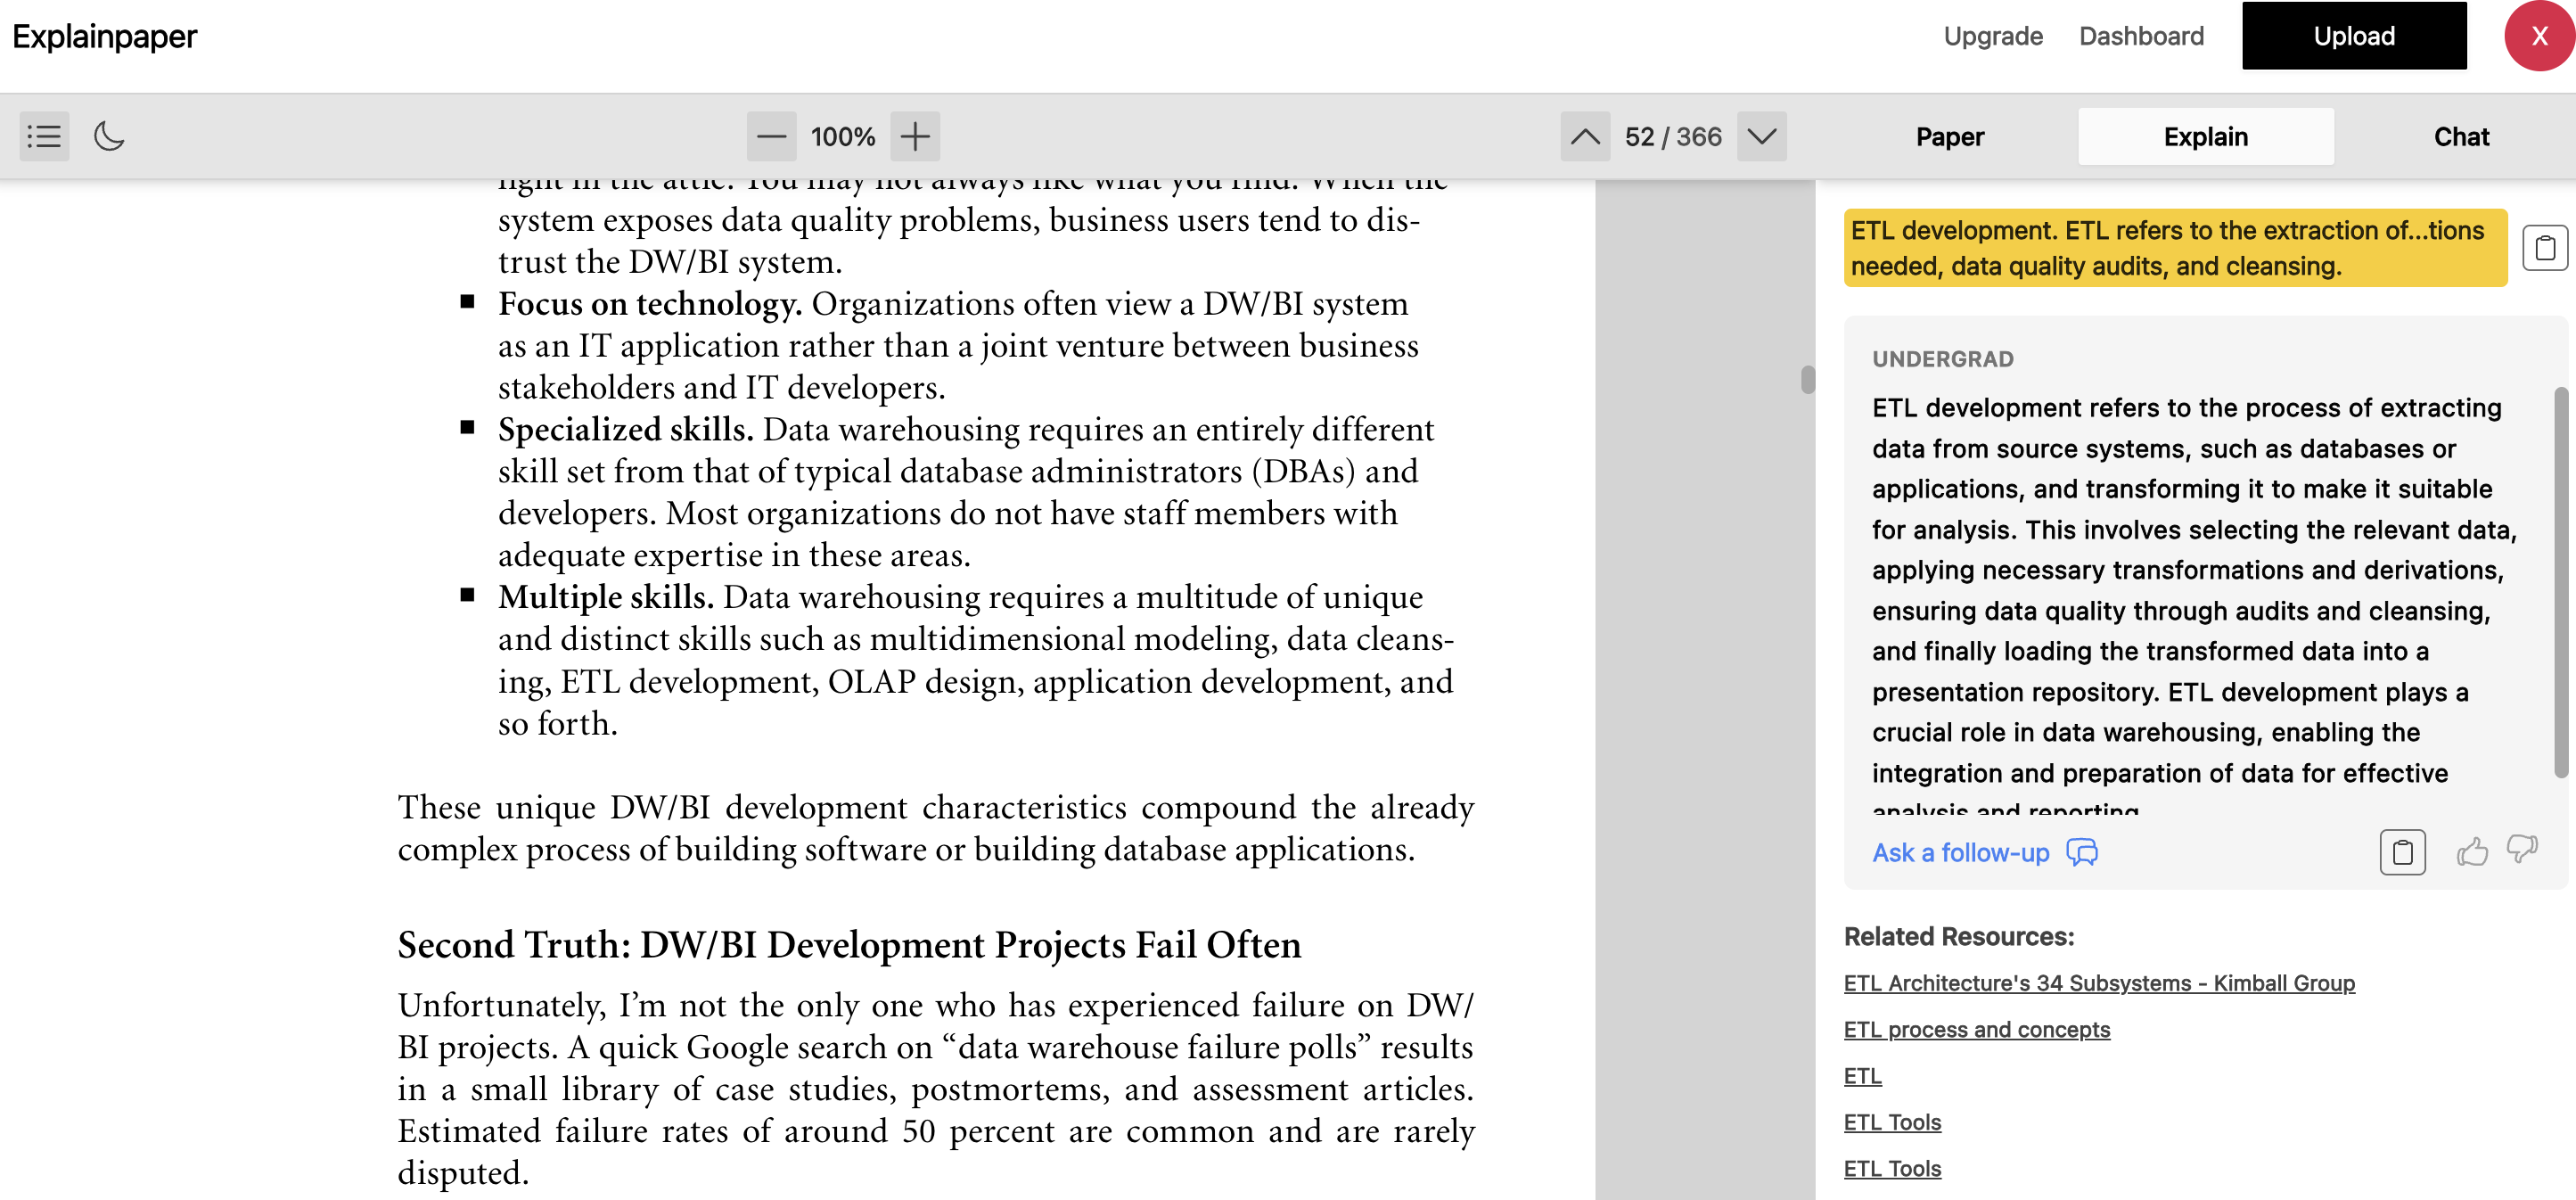
\includegraphics[width=0.9\linewidth]{Explainpaper_Example} 

}

\caption{Example of what Explainpaper can be used for}\label{fig:unnamed-chunk-12}
\end{figure}

\hypertarget{github-copilot}{%
\section{GitHub Copilot}\label{github-copilot}}

\href{https://github.com/features/copilot}{GitHub Copilot} is an AI developer tool that has gained significant recognition and was widely adopted within the programming community. Developed through a collaborative effort involving GitHub, OpenAI, and Microsoft, GitHub Copilot is a powerful tool that utilizes a generative AI model trained on extensive lines of code. Its primary function is to offer coding suggestions in multiple programming languages by interpreting natural language prompts.

\begin{figure}

{\centering 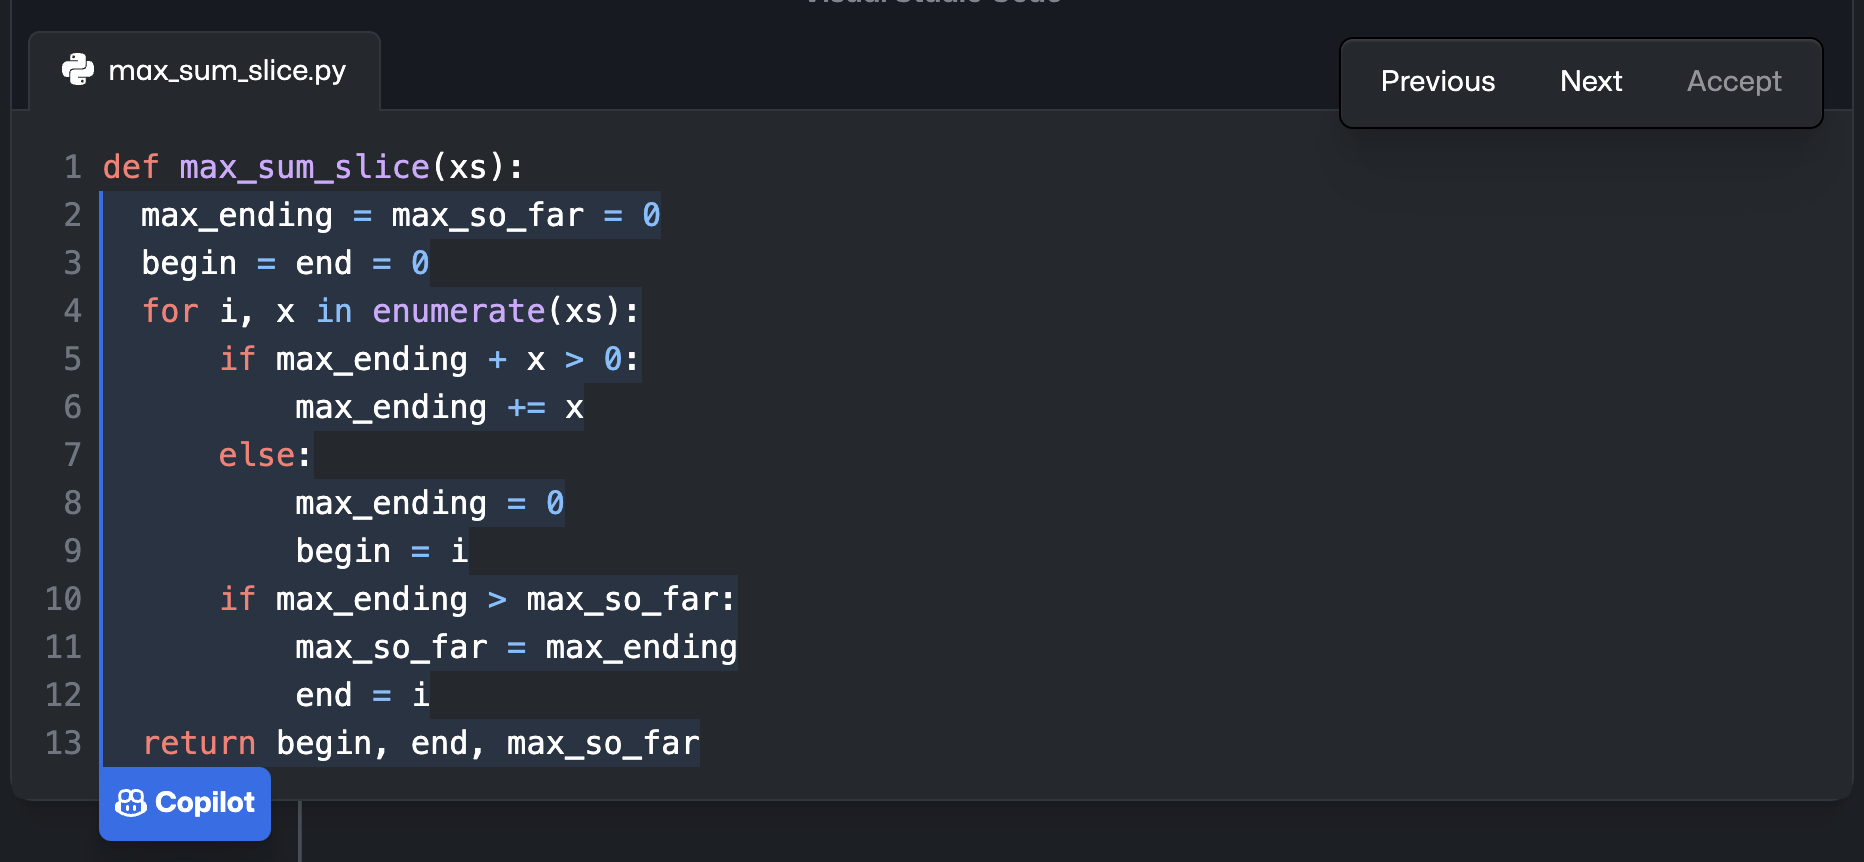
\includegraphics[width=0.95\linewidth]{GitHub_Copilot_Example} 

}

\caption{Example usage of GitHub Copilot}\label{fig:unnamed-chunk-13}
\end{figure}

\hypertarget{goblin-tools}{%
\section{Goblin Tools}\label{goblin-tools}}

\href{https://goblin.tools/}{Goblin Tool} offer a comprehensive solution for developers seeking guidance on difficult programming tasks. This tool utilizes its expertise to break down complex processes into manageable stages, which ensures that developers can follow a clear and structured path to successful implementation.

\begin{figure}

{\centering 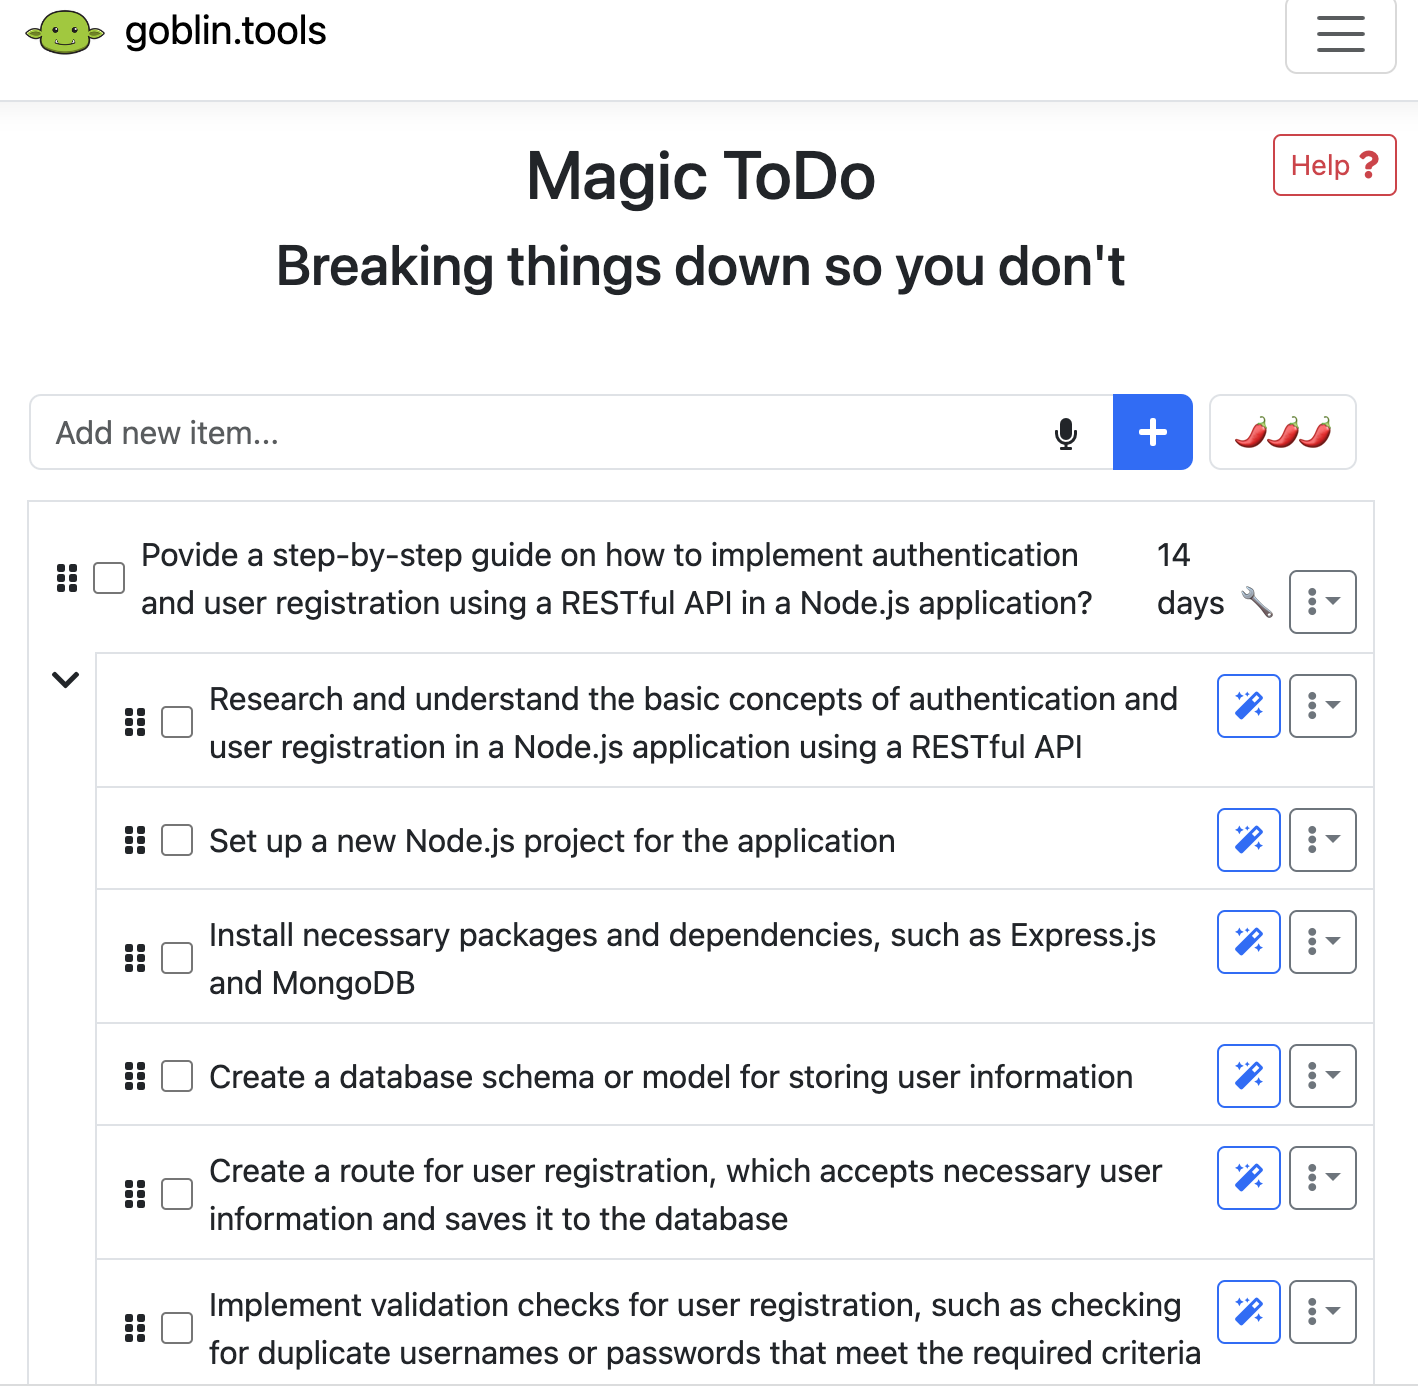
\includegraphics[width=0.7\linewidth]{Goblin_Tool_Example} 

}

\caption{Example of a programming task fed to Goblin Tool}\label{fig:unnamed-chunk-14}
\end{figure}

\hypertarget{dall-e}{%
\section{DALL-E}\label{dall-e}}

\href{https://labs.openai.com/}{DALL-E} is an advanced AI system developed by OpenAI that specializes in creating realistic images and art based on natural language descriptions. Users can provide text description of scenes, concepts or attributes and DALLE can translate these descriptions into images.

\begin{figure}

{\centering 
\includegraphics[width=0.7\linewidth]{Girl_with_a_pearlearrring_a_snake} 

}

\caption{"Girl with a pearl earring and a snake" by Johannes Vermeer}\label{fig:unnamed-chunk-15}
\end{figure}

\hypertarget{gen-1-runway-ml}{%
\section{Gen-1 Runway ML}\label{gen-1-runway-ml}}

\href{https://runwayml.com/}{Runway ML} allows users to transform text into video, create images from prompts, expand and re-image images, train custom AI models, manipulate videos, apply slow-motion effects, and so on.

\url{....}

\hypertarget{aiva}{%
\section{AIVA}\label{aiva}}

\href{https://www.aiva.ai/}{AIVA} is an AI tool designed to assist individuals in composing emotional and engaging soundtracks. It offers a range of predefined music styles like Modern, Pop, Rock, Jazz, etc. and to compose music. The platform offers a user-friendly interface that allows users to input specific parameters and preferences like style, mood and instrumentation and then generate original music that aligns with those criteria.

\begin{figure}

{\centering 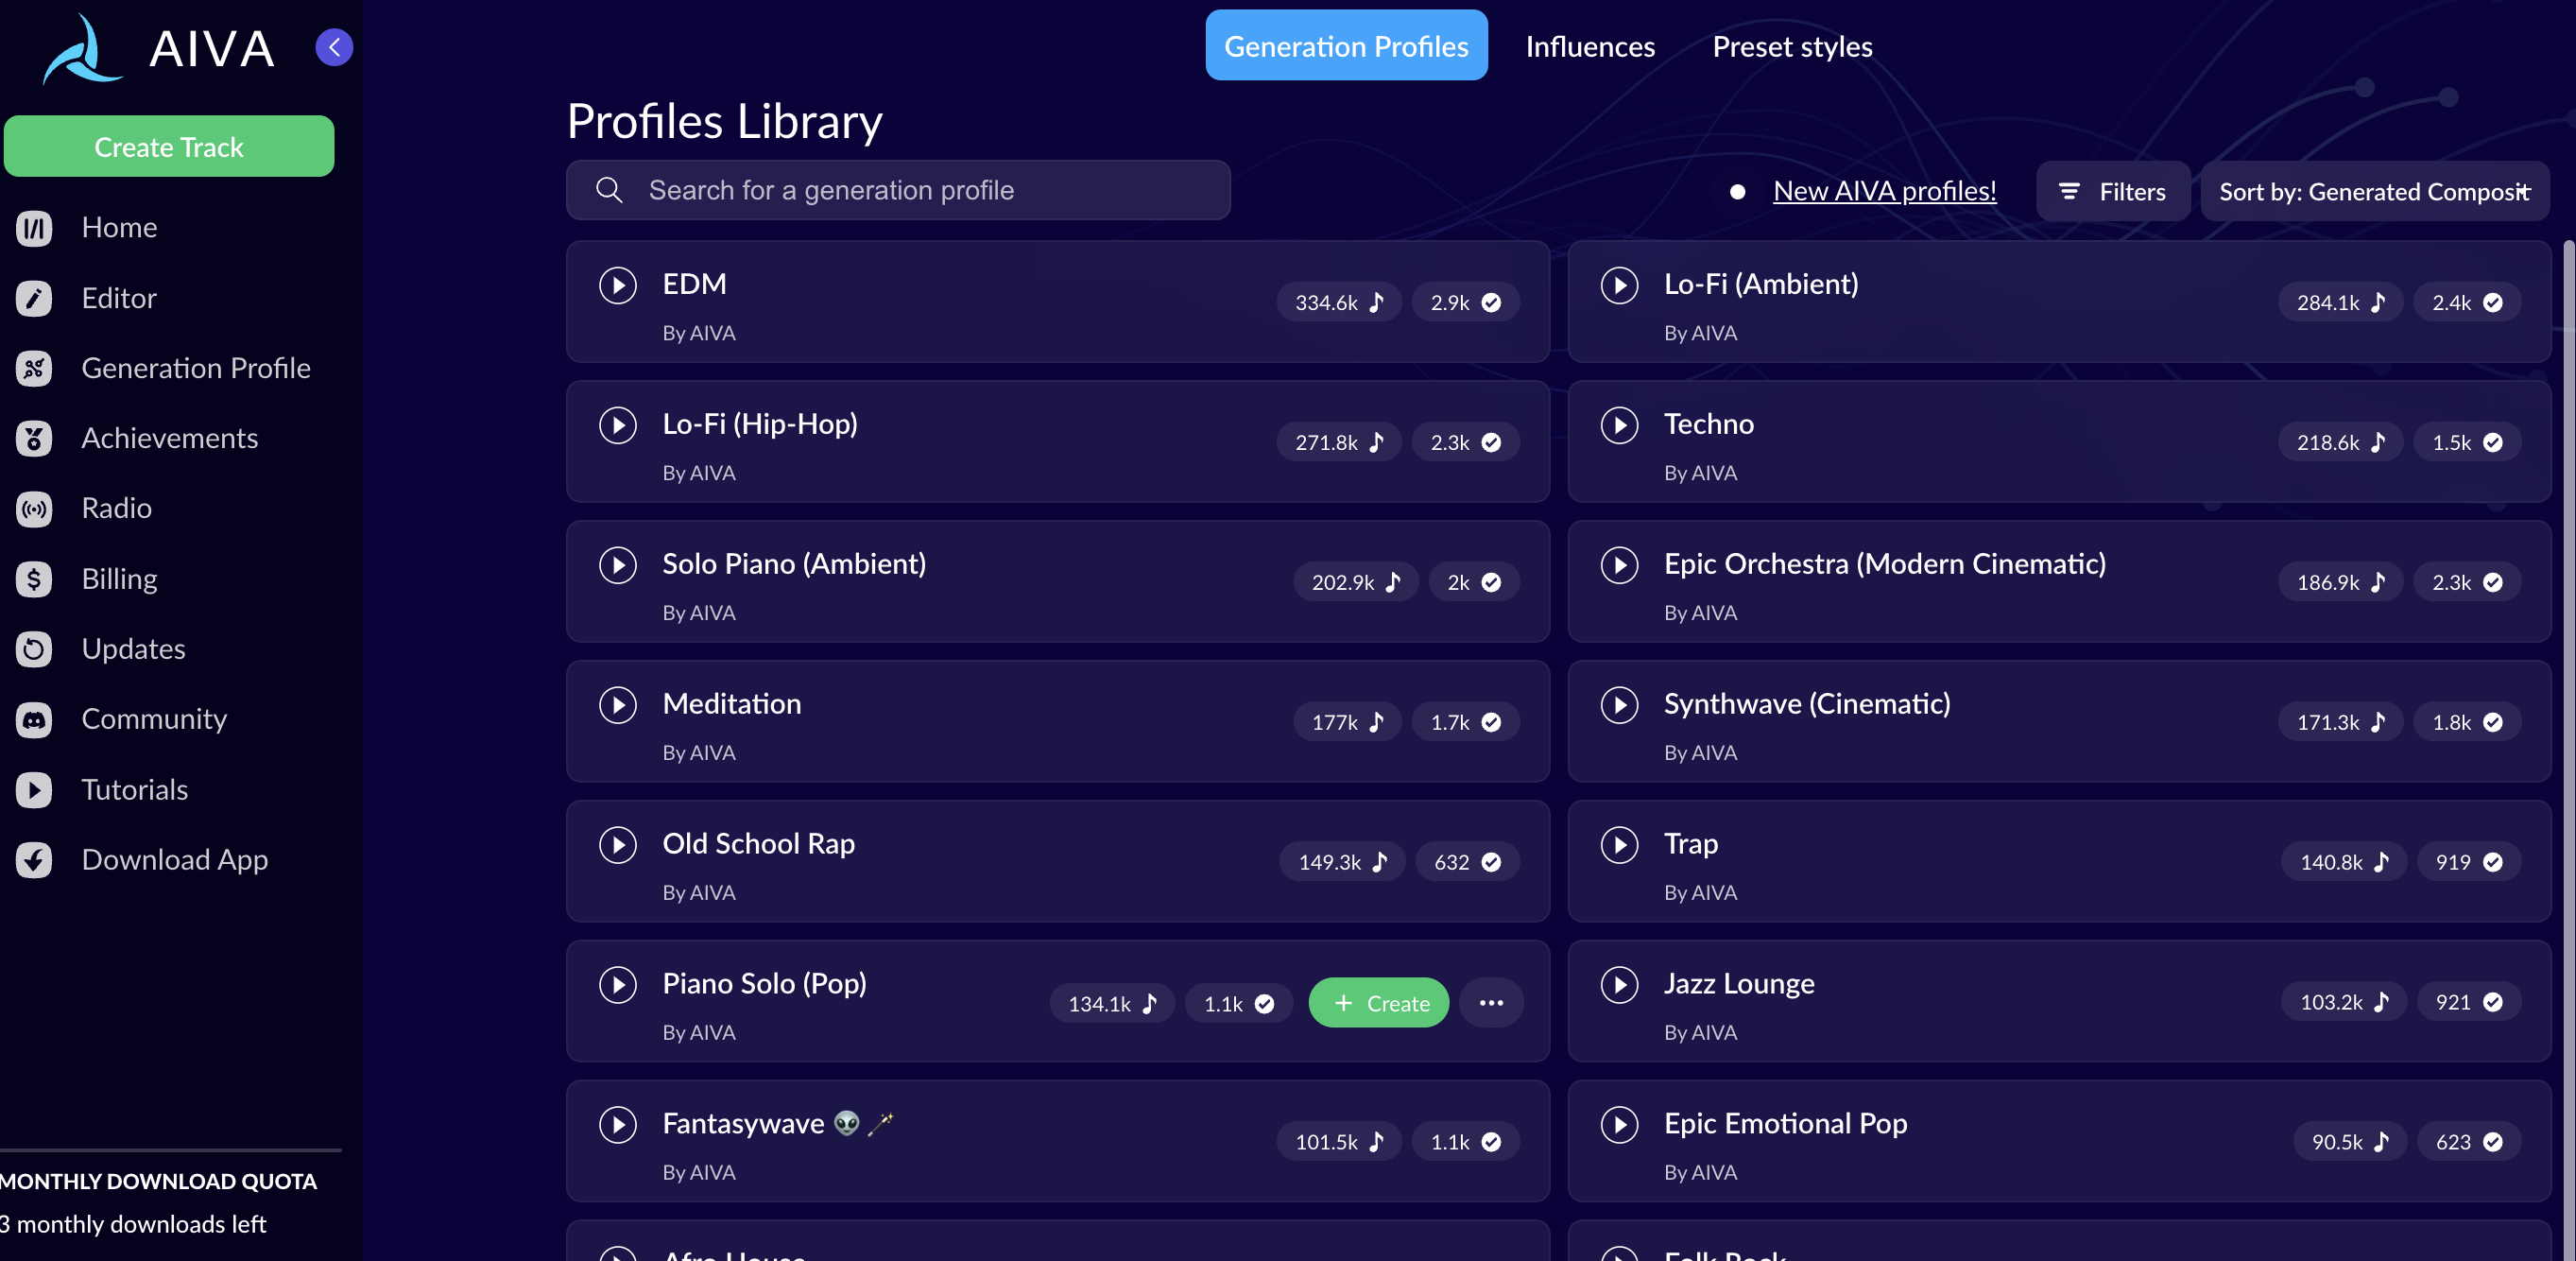
\includegraphics[width=0.95\linewidth]{AIVI_Dashboard} 

}

\caption{AIVI Dashboard}\label{fig:unnamed-chunk-17}
\end{figure}

\hypertarget{final-thoughts}{%
\chapter{Final Thoughts}\label{final-thoughts}}

The potential of Generative Artificial Intelligence is here. This report delves into the transformative influence of GenAI on business education, drawing insights from extensive faculty and staff interviews, exploring the capabilities of particular GenAI tools, and contextualizing them within the broader framework of university policies through the findings of the GAIA committee.

The insights gathered from interviews with faculty and staff highlight the diversity of perspectives surrounding the use of AI tools in education. While some embrace its potential to reshape teaching and engagement, others raise valid concerns about academic integrity and the need for a balanced approach. The disparity between faculty members who embrace AI's potential and those who exhibit caution underscores the need for ongoing dialogue and collaboration. This will foster an environment where educators collectively shape the future of education, leveraging AI to elevate critical thinking, problem-solving, and creativity among students. As AI technologies continue to advance, it is imperative for the Ross School of Business to establish a collaborative discourse, promoting an atmosphere that allows for a unified approach to this groundbreaking technology.

Our investigation into the GAIA committee's findings underscores the University of Michigan's proactive stance in understanding and regulating the integration of GenAI into its educational framework. The emergence of a UMich-based ChatGPT competitor further exemplifies the institution's commitment to innovation and adaptability. It is essential for the University to continue fostering an environment that encourages experimentation and collaboration to effectively harness the potential of AI in a responsible and constructive manner.

This discussion of AI between educators and students alike at the University of Michigan must emphasize a balanced and informed approach to its integration---one that prioritizes a modern education for students while also maintaining academic integrity standards assumed by instructors. By establishing guidance that helps the community navigate the complexities of AI while also capitalizing on the vast opportunities that it presents within education, the Ross School of Business can initiate an era of education that is both enriched and elevated by the transformative power of GenAI.

\hfill\break

\end{document}
